\documentclass[a4paper,UKenglish,cleveref, autoref, thm-restate]{lipics-v2021}
%This is a template for producing LIPIcs articles. 
%See lipics-v2021-authors-guidelines.pdf for further information.
%for A4 paper format use option "a4paper", for US-letter use option "letterpaper"
%for british hyphenation rules use option "UKenglish", for american hyphenation rules use option "USenglish"
%for section-numbered lemmas etc., use "numberwithinsect"
%for enabling cleveref support, use "cleveref"
%for enabling autoref support, use "autoref"
%for anonymousing the authors (e.g. for double-blind review), add "anonymous"
%for enabling thm-restate support, use "thm-restate"
%for enabling a two-column layout for the author/affilation part (only applicable for > 6 authors), use "authorcolumns"
%for producing a PDF according the PDF/A standard, add "pdfa"

%\pdfoutput=1 %uncomment to ensure pdflatex processing (mandatatory e.g. to submit to arXiv)
%\hideLIPIcs  %uncomment to remove references to LIPIcs series (logo, DOI, ...), e.g. when preparing a pre-final version to be uploaded to arXiv or another public repository
\usepackage{stmaryrd}
\usepackage{tikz}
\usetikzlibrary{shapes,arrows}
\usetikzlibrary{intersections}
\usetikzlibrary{automata}
\usetikzlibrary{positioning}
%\graphicspath{{./graphics/}}%helpful if your graphic files are in another directory

\bibliographystyle{plainurl}% the mandatory bibstyle

\title{Certified Symbolic Transducer with the Application of String Solver} %TODO Please add

%\titlerunning{Dummy short title} %TODO optional, please use if title is longer than one line

\author{Shuanglong Kan}{Barkhausen Institut, Germany \and \url{https://github.com/ShlKan} }{shuanglongkan@gmail.com}{https://orcid.org/0000-0002-1825-0097}{(Optional) author-specific funding acknowledgements}%TODO mandatory, please use full name; only 1 author per \author macro; first two parameters are mandatory, other parameters can be empty. Please provide at least the name of the affiliation and the country. The full address is optional. Use additional curly braces to indicate the correct name splitting when the last name consists of multiple name parts.



\authorrunning{S. Kan} %TODO mandatory. First: Use abbreviated first/middle names. Second (only in severe cases): Use first author plus 'et al.'

\Copyright{Jane Open Access and Joan R. Public} %TODO mandatory, please use full first names. LIPIcs license is "CC-BY";  http://creativecommons.org/licenses/by/3.0/

\ccsdesc[100]{\textcolor{red}{Replace ccsdesc macro with valid one}} %TODO mandatory: Please choose ACM 2012 classifications from https://dl.acm.org/ccs/ccs_flat.cfm 

\keywords{Dummy keyword} %TODO mandatory; please add comma-separated list of keywords

\category{} %optional, e.g. invited paper

\relatedversion{} %optional, e.g. full version hosted on arXiv, HAL, or other respository/website
%\relatedversiondetails[linktext={opt. text shown instead of the URL}, cite=DBLP:books/mk/GrayR93]{Classification (e.g. Full Version, Extended Version, Previous Version}{URL to related version} %linktext and cite are optional

%\supplement{}%optional, e.g. related research data, source code, ... hosted on a repository like zenodo, figshare, GitHub, ...
%\supplementdetails[linktext={opt. text shown instead of the URL}, cite=DBLP:books/mk/GrayR93, subcategory={Description, Subcategory}, swhid={Software Heritage Identifier}]{General Classification (e.g. Software, Dataset, Model, ...)}{URL to related version} %linktext, cite, and subcategory are optional

%\funding{(Optional) general funding statement \dots}%optional, to capture a funding statement, which applies to all authors. Please enter author specific funding statements as fifth argument of the \author macro.

\acknowledgements{I want to thank \dots}%optional

%\nolinenumbers %uncomment to disable line numbering



%Editor-only macros:: begin (do not touch as author)%%%%%%%%%%%%%%%%%%%%%%%%%%%%%%%%%%
\EventEditors{John Q. Open and Joan R. Access}
\EventNoEds{2}
\EventLongTitle{15th Conference on
Interactive Theorem Proving (ITP 2025)}
\EventShortTitle{ITP 2025}
\EventAcronym{ITP}
\EventYear{2025}
\EventDate{July 24--27, 2025}
\EventLocation{Little Whinging, United Kingdom}
\EventLogo{}
\SeriesVolume{42}
\ArticleNo{23}
%%%%%%%%%%%%%%%%%%%%%%%%%%%%%%%%%%%%%%%%%%%%%%%%%%%%%%

\lstset{
	basicstyle=\ttfamily,
	keywordstyle=\color{blue}\bfseries,
	keywords={definition,if,then,else, where, record, fun, lemma, type_synonym, fixes, assumes, shows},
	escapeinside={|}{|}
}

\begin{document}

\maketitle

%TODO mandatory: add short abstract of the document
\begin{abstract}
Finite-State Automata (FAs) and Finite-State Transducers (FTs) are integral components in the domains of programming languages and software engineering. Regular expressions, which are often implemented using FAs, play a pivotal role in languages such as JavaScript and Python. FTs extend the capabilities of FAs by allowing transformations of input strings into output strings, thus providing a more expressive framework for operations that involve both recognition and transformation. Despite the popularity of formalizing FAs and FTs within proof assistants like Coq and Isabelle/HOL, these formalizations frequently fall short in terms of applicability to real-world scenarios.

One limitation of traditional finite-state models is that transition labels are typically restricted to single characters from a finite alphabet. For example, a transition is often represented as $q \xrightarrow{a} q'$, where $a$ is a single character. However, in real-world applications, the alphabet of a FA or FT can be vast or even \emph{infinite}. This conventional approach to defining transitions can lead to a phenomenon known as transition explosion, where the number of transitions becomes unmanageably large.


A more pragmatic approach involves the formalization of symbolic FAs [1] and FTs [2], wherein transition labels are symbolic and potentially infinite. While the formalization of symbolic FAs has been comprehensively explored in the work of \cite{cpp/KanLRS22}, the formalization of symbolic FTs remains largely unexplored. This gap presents additional challenges in establishing the correctness and applicability of such formalizations.

In this paper, we endeavor to address this gap by presenting a formalization of symbolic transducers within the Isabelle/HOL framework. This formalization is refinement-based and is designed to be extensible with various symbolic representations of transition labels. To evaluate its effectiveness and efficiency, we applied this formalization to an SMT string solver for modeling replacement operations. The experimental results demonstrate that the formalized symbolic transducer can efficiently solve string constraints.


\end{abstract}

\section{Introduction}
\label{sec:introduction}

Automata and Transducers are crucial concepts in formal languages and have widely applications in programming languages and software engineering. For instance, [1] has shown the correspondence between  regular expressions in modern regular expressions and variants of FAs and FTs. Other industrial usage of FAs and FTs is AWS access control polices checking.


Even though there various  formalization of FAs and FTs in Coq, Isabelle, and other proof assistants. They are mainly based on classic definitions of FAs and FTs.  There some drawbacks when come to practical applications. (1) transition labels are 
non-symbolic and usually finite.
A classic and normal definition of a transition is $q\xrightarrow{a}q'$, where $a$ is a character in an finite alphabet.  This simple way will yield transition explosions. 
For instance, if the alphabet $\Sigma$ is of the size $10,000$, then a transition from $q$ to $q'$ that accept any characters in $\Sigma$ need to split into $10,000$ transitions. Automata product in this way will be very inefficient. Moreover, 
The alphabet are usually finite. For practical applications, infinite alphabet are often necessary. For instance, if the alphabet is all integers. 



Symbolic FAs and FTs [2,3,4] are extensions of classic FAs and FTs that make their application more practical. The transition labels are represented by algebra. For instances, intervals ($'a'-'z'$), boolean algebras ($x \% 2 == 0$), or others. This symbolic way is more succinct and its support for infinite alphabet extend the expressive power of FAs and FTs.

Formalizing FAs and FTs in Isabelle/HOL, Coq, and other proof assists are more challenging compare with formalizing classic ones. Moreover, how to make the formalization extensible is also an important point to think, because, symbolic FAs and FTs support different algebras symbolic representations. For new algebra representations, we do not want repeat some proof works.


Fortunately, symbolic FAs has been formalized in Isabelle/HOL [certistr] and experiments in [certistr] illustrates the efficiency and effective of symbolic FAs. Unfortunately FTs are not formalized yet.  FTs are more powerful and expressive than symbolic FAs. For instance, when FTs are support, replacement operation in modern programming languages, such as Javascript, python and others can be modelled as FTs. And CertiStr can be extended to support replacement operations.

In this paper, we formalize symbolic FTs based on symbolic FAs. In order to solve the potential extension problem of FTs to support additional transition label theories, the formalization is refinement-based, in which at the abstraction level, transition labels are modeled as a general concept: sets. We can project any theory to sets. \emph{extend this}.
The most important operation that we formalized and proved is the application operation on an input language.  More precisely, given an FA $\mathcal{A}$ (to represent a regular language) as the input language and a FT $\mathcal{T}$, the application operation $\mathcal{F}~\mathcal{A}$ is the  of output languages of FT after receiving the input language 

In the next refinement level, the states and transitions are stored in efficient data structure based on Isabelle/HOL refinement framework [2].
For transition labels, we implemented an interval algebra, which are efficient for creating, checking, interaction.
%
In the future the refinement of transition label from sets to other algebras instead of intervals can be done easily by implementing the common interfaces with interval algebras.

We highlight our formulization with the following points.
(1) Efficiency, the algebraic representation
support compressed storage of transition labels and efficiency checking
of membership.
(2) Extensible, the refinement based formulization allows the extension
of the SNFA to support different theories of transition labels.

The paper is organized as follows.
Section 2 presents the formalization of symbolic FTs.
Section 3 presents the Core operations of symbolic FTs.





\section{Formalization of Symbolic FTs}


We first present a pure mathematical form of SFTs \cite{VeanesHLMB12Transducer}, which is independent of Isabelle's formalization. 
The central concept is the label theory, which characterizes the process by which output labels are derived from input labels.

Let $\mathcal{U}$ be a multi-sorted carrier set or background universe, which is equipped with functions and relations over the elements. We use $\tau$ as a sort and $\mathcal{U}^\tau$ denotes the sub-universe of elements of type $\tau$. 
We have a special type $\mathbb{B}$ with $\mathcal{U}^\mathbb{B} = \{ \top, \bot\}$, which corresponds to the boolean type. Assume $\mathbb{N}$ is the set of elements of the sort natural numbers.

A lambda term is defined as $\lambda x. t$ of the type $\tau_1 \rightarrow \tau_2$.
When $\tau_2$ is $\mathbb{B}$, this lambda term is a predicate. Assume $\psi$ is a predicate. We write $a\in \llbracket\psi \rrbracket$ if $\psi~a=\top$. For the non-predicate lambda term, we view it as a function, which generates an output element of type $\tau_2$ with the input term of type $\tau_1$. 
With these notations and the above definitions, we can define SFTs as follows.

\begin{definition}[Symbolic Finite Transducer]
\label{def-sft}
   A Symbolic Finite Transducer over $\tau_1\rightarrow \tau_2$ is a quadruple $\mathcal{T} = (\mathcal{Q}, \Delta, \mathcal{I}, \mathcal{F})$, where 
   \begin{itemize}
   \item $\mathcal{Q}$ is a finite set of states,
   \item $\mathcal{I}\subseteq \mathcal{Q}$ is the set of initial states,
   \item $\mathcal{F} \subseteq\mathcal{Q}$ is the set of accepting states,
   \item $\Delta$ is the set of transition relations. Each element in $\Delta$ is of the form $(q, \psi, f, q') \text{ or}$ $\text{written in }q\xrightarrow{\psi, f} q'$, where $q$ and $q'$ are the states in $\mathcal{Q}$.
   $\psi$ is a predicate of type $\tau_1\rightarrow \mathbb{B}$.
   $f$ is a lambda term of the type $\tau_1\rightarrow \tau_2$. $f$ is called "output function".
   \end{itemize}

For each transition $q\xrightarrow{\phi, f} q'$, if there exists an element $a\in \llbracket \phi \rrbracket$, where $a$ is called an input,  then the application $(f~a)$ is the output.
   
\end{definition}

SFTs accept an input word and generate an output. This can be defined by \emph{runs} of SFTs.
An SFT run $\sigma$ is a sequence $(q_0, \psi_0, f_0, q_1),(q_1, \psi_1, f_1, q_2),\ldots, (q_{n-1}, \psi_{n-1}, q_n)$ such that $q_0\in \mathcal{I}$ and $(q_i, 
\psi_i, f_i, q_{i+1}), 0 \leq i \leq n-1$ is a transition in $\Delta$.
$\sigma$ is an accepting run when $q_n$ is an accepting state.

For a word $w = a_0,\ldots, a_{n-1}$, it is accepted by $\sigma$ iff $a_i \in \llbracket\psi_i \rrbracket$ for $0 \leq i \leq n - 1$. Run $\sigma$ will generate an output sequence if $w$ is accepted by it, which is $w'= (f_0~a_0), \ldots (f_{n_1}~a_{n_1})$. We call in the sequent:
\begin{itemize}
\item  $(a_0,(f_0~a_0)), \ldots, (a_{n-1},(f_{n-1}~a_{n-1}))$ a \emph{path},
\item $a_0,\ldots,a_{n-1}$ the \emph{input} of the path and $(f_0~a_0), \ldots, (f_{n-1}~a_{n-1})$ the \emph{output} of the path.
\end{itemize}

If $a_0,\ldots,a_{n-1}$ is accepted by an accepting run in $\mathcal{T}$, we say that the path is an accepting path of $\mathcal{T}$.
For a path $\pi$, we denote the input of $\pi$ as $in(\pi)$ and the output of $\pi$ as $out(\pi)$.
%
Given an SFT $\mathcal{T}$ and a word $w$, we define the operation product of $\mathcal{T}$ and $w$ (denoted as $\mathcal{T}\times\{w\}$) as the set of outputs generated by $\mathcal{T}$ with the input $w$. More precisely, 
\[
\mathcal{T}\times\{w\} = \{w'\mid \exists \pi.~\pi \text{ is an accepting path }\land in(\pi) = w \land out(\pi) = w'\}.
\]

To make the operation \emph{product} more general, we extend the operation to an SFT and a set of intput words represented by a regular language, which can be denoted as an NFA. More precisely,
\[
\mathcal{T}\times\{\mathcal{A}\} = \{w'\mid w.~w\in \mathcal{L}(\mathcal{A})\land w' = \mathcal{T}\times\{w\} \}, \text{where $\mathcal{L}(\mathcal{A})$ denotes the language of $\mathcal{A}$}.
\] 

\begin{figure}[hbt!]
  \centering
  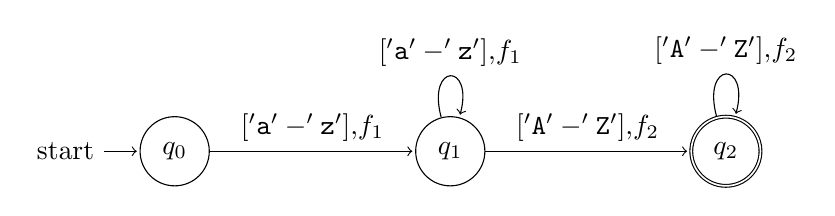
\begin{tikzpicture}[shorten >=1pt, node distance=3.5cm, on grid, auto]
    \node[state, initial] (q_0)   {$q_0$}; 
    \node[state] (q_1) [right=of q_0] {$q_1$}; 
    \node[state, accepting] (q_2) [right=of q_1] {$q_2$}; 
 
    \path[->] 
    (q_0) edge node {[$'\texttt{a}'-'\texttt{z}'$],$f_1$} (q_1)
    (q_1) edge node {[$'\texttt{A}'-'\texttt{Z}'$],$f_2$} (q_2)
    (q_1) edge[loop above] node {[$'\texttt{a}'-'\texttt{z}'$],$f_1$} (q_1)
    (q_2) edge[loop above] node {[$'\texttt{A}'-'\texttt{Z}'$],$f_2$} (q_2);
 \end{tikzpicture}
    \caption{The formalization of $FTs$ in Isabelle/HOL}
    \label{fig-example-ft}
    \end{figure}   
We now illustrate SFTs with an example in Figure \ref{fig-example-ft}. It accepts strings of the regular expression $/['\texttt{a}'-'\texttt{z}']+['\texttt{A}'-'\texttt{Z}']+/$. 
It uses intervals $[i-j]$ as the input label, which is a predicate that returns true if the input letter is between $i$ and $j$.
The function $f_1=\lambda x.~ \texttt{toUpper}(x)$ maps each lowercase letter to uppercase letter, and $f_2=\lambda x.~\texttt{toLower}(x)$ maps each uppercase letter to lowercase letter.
Give an string "$\texttt{bigSMALL}$", the SFT will generate an output "$\texttt{BIGsmall}$". 






\subsection{The Isabelle/HOL Formalization of SFTs}

\begin{figure}[hbt!]
	\begin{lstlisting}
record (|$'q,$||$~'a,$| |$'b$|) |$\mathbf{NFT}$| =
	|$\mathcal{Q}_T$| :: "|$'q$| set"
	|$\Delta_T$| :: "(|$'q,$||$~'a,$| |$'b$|) LTTS"
	|$\mathcal{I}_T$| :: "|$'q$| set"
	|$\mathcal{F}_T$| :: "|$'q$| set"
        |$\mathcal{M}$| :: "|$'b\Rightarrow 'a$| Tlabel"
        
type_synonym |$('q, 'a, 'b)$| LTTS = "|$('q \times ('a \text{ set option }\times b) \times 'q)$| set"

type_synonym |$'a$| Tlabel = "|$'a \text{ option} \Rightarrow 'a$ set"
	\end{lstlisting}
\caption{The formalization of $FTs$ in Isabelle/HOL}
\label{fig-def-FT}
\end{figure}

Figure \ref{fig-def-FT} shows our formalization of SFTs in Isabelle / HOL. The elements $\mathcal{Q}$, $\mathcal{I}$, and $\mathcal{F}$ are intuitive when referring to Definition \ref{def-sft}. However, the transitions are not exactly the same. 
%
The set of transitions is defined by \texttt{LTTS} ( which is short for Labeled Transducer Transition System). Each transition is defined as $'q \times ('a \text{ set option }\times b) \times 'q$. There are some design decisions, which are made to make the FT formalization more abstract and flexible.

Firstly, $'a \text{ set option }$ is the input type of the transition, it accepts a set of elements of type $'a$ or \texttt{None} regarding the semantics of the type \texttt{option}. 
Accepting a set of $'a$ elements aims to express the same but more abstract semantics of the input labels in Definition \ref{def-sft}, in which an input label is a predicate. A predicate's semantics as introduced before represents a set of elements that make the predicate true. But predicates have various different forms. For instance, the interval $[1, 9]$ is a predicate that contains all elements $e$ between $1$ and $9$, i.e., $1 \leq e \leq 9$. The predicate $\lambda x : \mathbb{N}.~ x \text{ mod } 2 = 0$ denotes the set of even natural numbers. All these different forms of labels are abstracted as sets in the formalization.

%
The value $\texttt{None}$ is used to denote $\varepsilon$-move, that is, it accepts nothing but may still output some elements. This design makes it easier model real world applications in FTs. We will show an example after introducing the output functions. 

The second element of type $'b$ is the \emph{indexes} of the output functions.  $\mathcal{M}$ maps each of these indexes to an output function. The output function, defined by \texttt{Tlabel} maps a single input element to a set of output elements instead of single one. The reason is to allow FTs output non-deterministically, which means that the output may randomly or according to some criteria select one of the element in the set to output.

Now let us look at an example. In some modern programming languages, there are support for replacement operations : $\texttt{replace}(\texttt{str}, \texttt{pattern}, \texttt{replacement})$. This operation replaces the first occurrence of the substring  in \texttt{str} that matches \texttt{pattern} (which usually a regular expression) with the string \texttt{replacement}). 
We can easily model this operation using our formalization of NFTs with the following steps:
\begin{itemize}
\item Step 1, construct a corresponding NFA from \texttt{pattern}).
\item Step 2, convert each transition label for transducers by adding a function that maps each input character to empty, that is, generate nothing.
\item Step 3, Add a new accepting state, and redirect existing accepting states to the new accepting state and transition label as $(\texttt{None}, \lambda x. \texttt{replacement})$.
\item Step 4, unlabel previous accepting states as non-accepting states. 
\end{itemize}

We can see that the definition of transition labels in NFTs makes it is very easy to model the replacement operation.

\section{The Product Operation of NFTs}
\label{sec-form-fts}

Given an NFT $\mathcal{N}$ and a word $w$, it is crucial and interesting that the possible output words can be calculated. This is the operation, we want to formalize, but we will generalize this operation.

Instead of calculating the outputs for a single word, the operation calculates the outputs for a set of input words. Single word input is a special case with the set contains exactly only one element.

The set of input words is modeled as a regular language. To be more precise, let $\mathcal{N}$ be an NFT, and $\mathcal{A}$ be an NFA. We define the operation $\texttt{PRODUCT} ~\mathcal{N}~\mathcal{A} = \{w'\mid w\in \mathcal{L}(\mathcal{A})\text{ and } w' = \mathcal{N}~\mathcal{A}\}$, where $\mathcal{L}(\mathcal{A})$ denotes the language of NFA $\mathcal{A}$.


But there is one thing we need to consider, as our NFT formalization accepts $\varepsilon$-transitions, the output NFAs may contain $\varepsilon$-transitions as well. Unfortunately, [CertiStr] does not formalize $\varepsilon-$NFA. We formalize symbolic $\varepsilon-$NFA and the conversion from $\varepsilon-$NFA to NFA. We only present the definitions of $\varepsilon-$NFA and NFA in this paper. The more details including correctness proofs can be found in the Isabelle code. 

\begin{figure}[hbt!]
	\begin{lstlisting}
record (|$'q,$||$~'a$|) |$\mathbf{NFA}$| =
	|$\mathcal{Q}$| :: "|$'q$| set"
	|$\Delta$| :: "(|$'q,$||$~'a$|) LTS"
	|$\mathcal{I}$| :: "|$'q$| set"
	|$\mathcal{F}$| :: "|$'q$| set"

record (|$'q,$||$~'a$|) |$\mathbf{eNFA}$| =
	|$\mathcal{Q}_e$| :: "|$'q$| set"
	|$\Delta_e$| :: "(|$'q,$||$~'a$|) LTS"
        |$\Delta_e'$| :: "|$('q * 'q)$| set"
	|$\mathcal{I}_e$| :: "|$'q$| set"
	|$\mathcal{F}_e$| :: "|$'q$| set"

type_synonym |$('q, 'a)$| LTS = "|$'q \times 'a \text{ set }\times 'q$|"    
	\end{lstlisting}
\caption{The formalization of $\varepsilon-$NFA and NFA in Isabelle/HOL}
\label{fig-def-FAs}
\end{figure}

Figure \ref{fig-def-FAs} shows the definitions of NFA and $\varepsilon-$NFA.
The record type \texttt{eNFA} corresponds to $\varepsilon-$NFA. $\Delta_e$ is same as $\Delta$ in \texttt{NFA}. $\varepsilon$-transitions are defined by $\Delta_e'$.  Now we are ready to present the operation \emph{Product}. Let $\mathcal{T}$ be an SFT and  $\mathcal{A}$ be an NFA. The output language generated by $\mathcal{T}$ with the input language $\mathcal{A}$ is an an \texttt{eNFA} $\mathcal{A}'$. 

\begin{figure}[hbt!]
	\begin{lstlisting}
definition productT :: |$"('q,'a,'b,'c)"$| NFT |$\Rightarrow$| ('q,'a) NFA |$\Rightarrow$| 
           |$(('a,'b)$| Tlabel |$\Rightarrow 'a \text{ set}\Rightarrow 'b\text{ set option})\Rightarrow$|
           |$('q\times 'q, ~'b)$| eNFA where
  "productT |$\mathcal{T}$| |$\mathcal{A}$| F = |$\llparenthesis$|
    |$\mathcal{Q}e = \mathcal{Q}_t~\mathcal{T} \times \mathcal{Q} ~\mathcal{A}$|,
    |$\Delta_e = \{((p,p'),~\texttt{the }(((\mathcal{M}~\mathcal{T})~f)\texttt{ None}),~(q, p'))\mid p, p', q, f.~p'\in \mathcal{Q}~\mathcal{A} \land$|
          |$(p, (\texttt{None}, f), q)\in \Delta_T \mathcal{T} \land \exists S. (\mathcal{M}~\mathcal{T})~f~\text{None} = \text{Some } S\} ~\cup$|
        |$\{((p,p'),~\texttt{the }(F~((\mathcal{M}~\mathcal{T})~f)~(\sigma_1\cap\sigma_2)),~(q, q'))\mid p, p', q, \sigma_1, \sigma_2, q', f.~$|
          |$ (p, (\text{Some }\sigma_1, f), q)\in \Delta_T~\mathcal{T} \land (p', \sigma_2, q')\in\Delta~\mathcal{A}\land \sigma_1\cap \sigma_2 = \emptyset \land$|
            |$ \exists S.~F~((\mathcal{M}~\mathcal{T})~f)~(\sigma_1\cap\sigma_2) = \text{Some } S\}$|,
    |$\Delta_e' = \{((p,p'),~\text{the }(((\mathcal{M}~\mathcal{T})~f)\texttt{ None}),~(q, p'))\mid p, p', q, f.~p'\in \mathcal{Q}~\mathcal{A} \land$|
          |$(p, (None, f), q)\in \Delta_T~\mathcal{T} \land (\mathcal{M}~\mathcal{T})~f~\texttt{None} = \text{None}\} ~\cup$|
        |$\{((p,p'),~\texttt{the }(F~((\mathcal{M}~\mathcal{T})~f)~(\sigma_1\cap\sigma_2)),~(q, q'))\mid p, p', q, \sigma_1, \sigma_2, q', f.~$|
          |$ (p, (\text{Some }\sigma_1, f), q)\in \Delta_T~\mathcal{T} \land (p', \sigma_2, q')\in\Delta~\mathcal{A}\land \sigma_1\cap \sigma_2 = \emptyset \land$|
            |$ \exists x\in(\sigma_1\cap\sigma_2).~((\mathcal{M}~\mathcal{T})~f)~(\text{Some } x) = \text{None} \}$|,
    |$\mathcal{I}_e = \mathcal{I}_t~\mathcal{T} \times \mathcal{I}~\mathcal{A}$|
    |$\mathcal{F}_e = \mathcal{F}_t~\mathcal{T} \times \mathcal{F}~\mathcal{A}$| |$\rrparenthesis$|"
	\end{lstlisting}
\caption{The formalization of $\varepsilon-$NFA and NFA in Isabelle/HOL}
\label{fig-def-FTProd}
\end{figure}

Figure \ref{fig-def-FTProd} depicts the abstract level formalization for the product of an SFT and an NFA. The parameters $\mathcal{T}$ and $\mathcal{A}$ are intuitive. But we need to explain the role of \texttt{F}. The output function is of type "$'a \Rightarrow 'b \text{set option}$", which applies to a single element of the type $'a$. $\texttt{F}$ extends this function to apply it to a set of elements. More precisely, let $f$ be an output function, the semantics of $\texttt{F}$ is defined as $\texttt{F}~f~A=\bigcup_{a\in A} (\text{if }f~a= \text{Some }S \texttt{ then } S \texttt{ else } \emptyset)$.
The transition relations $\Delta_e$ and $\Delta_e'$ are defined by splitting into two cases, whether the transitions in SFTs are $\varepsilon$-transitions or not.

$\Delta_e$ has two cases:(1) when $(p, (\text{None}, f),  q)$ is a transition in the NFT. Because the input can be empty ($\varepsilon$), therefore the NFA does not need to move. Therefore the product transtion just output of $f~\text{None}$. (2) when $(p, (Some~\sigma_1, f), q)$ is a transition in the NFT. This transition can only synchronize with the transitions in the NFA that have shared characters with $\sigma_1$. And the output is $F~f~(\sigma_1\cap\sigma_2)$, where $\sigma_2$ is the input label of the NFA. Similarly, $\Delta_e'$ has two cases too.


To establish the correctness of the abstract definition of the product operation, we first formalize the outputs of a Non-deterministic Finite Transducer (NFT) with respect to the input of a Non-deterministic Finite Automaton (NFA). Figure \ref{fig-def-output} presents two key definitions: (1) \texttt{outputE}, which extracts the sequence of outputs $o_1, \ldots, o_n$ from a given NFT path $(i_1, o_1), \ldots, (i_n, o_n)$; and (2) \texttt{outputL}, which represents the set of all possible outputs generated by an NFT $\mathcal{T}$ for the input language defined by an NFA $\mathcal{A}$.


\begin{figure}[hbt!]
	\begin{lstlisting}
fun outputE :: "|$('a \text{ option} \times 'b \text{ option}) \text{ list} \Rightarrow 'b \text{ list}$|" where
  "outputE [] = []" |$\mid$|
  "outputE ((_, Some a) # l) = a # (outputE l)" |$\mid$|
  "outputE ((_, None) # l) = (outputE l)"

definition outputL :: "|$('q, 'a, 'b, 'c)\text{  NFT} \Rightarrow $|
            |$ ('c \Rightarrow ('a, 'b)\text{  Tlabel}) \Rightarrow 
                               ('q, 'a) \text{ NFA\_rec} \Rightarrow 'b\text{ list set}$|" where
  "outputL |$\mathcal{T}$| M |$\mathcal{A}$| = {outputE |$\pi~\mid~\pi~q~q'$|. |$q\in \mathcal{I}_T~\mathcal{T} \land q' \in \mathcal{F}_T~\mathcal{T} \land$|
                |$ \text{LTTS\_reachable }(\Delta_T~\mathcal{T})~\text{M}~q~\pi~q'\land \text{inputE }\pi\in \mathcal{L}~\mathcal{A}$|}" 
	\end{lstlisting}
\caption{The formalization of $\varepsilon-$NFA and NFA in Isabelle/HOL}
\label{fig-def-output}
\end{figure}


\begin{figure}[hbt!]
	\begin{lstlisting}
lemma productT_correct:
  fixes |$\mathcal{T}$| |$\mathcal{A}$| F
  assumes F_ok1: "|$\forall~f~s.~(\forall e \in s. f (\text{ Some } e) = \text{None}) \mapsto \text{ F}~f~s = \text{None}"$|
      and F_ok2: "|$\forall~f~s.~\text{F }f~s = $|
            |$\text{Some }(\cup \{\text{the }(f (\text{ Some }e))\mid e. e \in s \land f~(\text{Some }e) \neq \text{ None}\})$|"
      and wfTA: "NFT_wf |$\mathcal{T}~\land \text{ NFA } \mathcal{A}$|"
    shows "|$\mathcal{L}_e$| (productT |$\mathcal{T}~\mathcal{A}$| F) = outputL |$\mathcal{T}~(\mathcal{M}~\mathcal{T})~\mathcal{A}$|"

	\end{lstlisting}
\caption{The formalization of $\varepsilon-$NFA and NFA in Isabelle/HOL}
\label{fig-def-product-correct}
\end{figure}

Figure \ref{fig-def-product-correct} shows the correctness of the product operation and Figure \ref{fig-def-output} contains the definitions of \texttt{outputE} and \texttt{outputL} that are used in Lemma \texttt{productT\_correct}.
The two assumptions define the constraints of the function \texttt{F}.
The conclusion in \textcolor{blue}{\texttt{show}} illustrates 
that the language equivalence between the production definition and mathematical semantics.

\section{Algorithm Level Refinement}
\label{sec_alg_refinement}
In Section \ref{sec-form-fts}, we give an abstract definition of NFT's product operation. In this section, we present the possible way to compute the Product from programming language's perspective.
In this level, we will also refine the transition labels from \emph{sets} to interval algebra.

\subsection{Intervals}
An interval is defined as a pair $(i, j)$, which corresponds to the set $\{e \mid e \geq i \land e \leq j\}$. In our formalization, we extends the interval definition to a list, that is $[(i_1, j_1), \ldots, (i_n, j_n)]$, which corresponds to the set $\bigcup_{1\leq k\leq n}\{e \mid i_k \leq e \leq i_n\}$. This definition enables us to merge more transitions in NFAs. Moreover, when an interval operation produces more than two intervals, we do not need to split the intervals. For instance, the interval result of $(1, 5) - (3, 4)$ (the difference between the interval $[1, 5]$ and $[3, 4]$) is equivalent to $[(1, 2), (5, 5)]$.


In the sequent, intervals always mean interval lists.
There are a collection interfaces for intervals. 
\begin{enumerate}
  \item $\texttt{semI}~i$, formalize the semantics of an interval as a set, that is $\texttt{semI }(i,j) = \{e \mid e \geq i \land e \leq j\}$.
  \item $\texttt{emptyI}~i$, checks the emptiness of an interval.
   \item $\texttt{nemptyI}~i$, checks the non-emptiness of an interval.
  \item $\texttt{intersectIs}~i_1~i_2$, computes the intersection of two intervals.
  \item $\texttt{diffIs}~i_1~i_2$, computes the intervals difference, that is the interval corresponds to the set $\texttt{semI}(i_1)-\texttt{semI}(i_2)$.
\end{enumerate}

We define a canonical form for intervals to facilitate the proof. An interval $[i_1, j_1), \ldots, (i_n, j_n)]$ is in canonical form if 
(1) $i_k \leq j_k, 1 \leq k \leq n$,
(2) $j_k\leq i_{k+1}, 1 \leq k < n$.
All the interval operations are proved to keep the canonical form after the operation if the input intervals are in canonical form.




\subsection{Algorithm of Product Computation.}

Fig. \ref{fig-compute-nft-product} illustrates the product computation of a SFT and an SFA. \footnote{To make it easier to understand, the Isabelle code presented in this section is not exactly the same as the real one.}
\texttt{prods\_imp} computes the product of two sets. It is illustrated in \ref{fig-def-prods_imp}. We use the constructs from \emph{Refine\_Monadic}. \texttt{prods\_imp} itself is intuitive: the nested two loops traverse all possible combination of states in the states. 
The \texttt{FOREACH} construct in \emph{Refine\_Monadic} is similar to OCaml's \texttt{Set.fold}. $\texttt{FOREACH}~S~f~I$ traverses all elements in $S$ and applies $f$ of type $'a \Rightarrow 'b \Rightarrow 'b$ to each element. $I$ is the initial value of type $'b$.



\begin{figure}[hbt!]
	\begin{lstlisting}
definition productT_impl where
  "productT_impl |$\mathcal{T}$| |$\mathcal{A}$| F fe = do {
    Q |$\leftarrow$| prods_imp (nft_states |$\mathcal{T}$|) (nfa_states |$\mathcal{A}$|);
    (D1, D2) |$\leftarrow$| trans_comp_imp (nft_tranfun |$\mathcal{T}$|) F fe 
        (nft_trans |$\mathcal{T}$|) (nfa_trans |$\mathcal{A}$|) (nfa_states |$\mathcal{A}$|);
    I |$\leftarrow$| prods_imp (nft_initial |$\mathcal{T}$|) (nfa_initial |$\mathcal{A}$|);
    F |$\leftarrow$| prods_imp (nft_accepting |$\mathcal{T}$|) (nfa_accepting |$\mathcal{A}$|);
    RETURN (Q,D1,D2,I, F)
  }"
\end{lstlisting}
\caption{The computation of NFT product}
\label{fig-compute-nft-product}
\end{figure}



\begin{figure}[hbt!]
	\begin{lstlisting}
definition prods_imp where
  "prods_imp Q1 Q2 =
   FOREACH {q. q |$\in$| Q1} (|$\lambda$| q Q. do {
    S |$\leftarrow$| FOREACH {q. q |$\in$| Q2}
         (|$\lambda$| q|$'$| Q|$'$|. RETURN ({(q,q|$'$|)} |$\cup$| Q|$'$|)) |$\emptyset$|;
    RETURN (Q |$\cup$| S)
   }) |$\emptyset$|"
\end{lstlisting}
\caption{The formalization of $\varepsilon-$NFA and NFA in Isabelle/HOL}
\label{fig-def-prods_imp}
\end{figure}



\begin{figure}[hbt!]
	\begin{lstlisting}
definition trans_comp_imp where
  "trans_comp_imp M F T1 T2 Q =
    FOREACH {t. t |$\in$| T1}
      (|$\lambda$| (q, (|$\alpha$|, f), q|$'$|) (D1, D2). 
        (if (|$\alpha$| = None) then 
          (subtrans_comp_|$\varepsilon$| M q  f q|$'$| F T2 D1 D2)
        else 
          (subtrans_comp M q (the |$\alpha$|) f q|$'$| F T2 D1 D2)
      )) (|$\emptyset$|, |$\emptyset$|)"
\end{lstlisting}
\caption{The computation of transition sets}
\label{fig-def-prods-imp}
\end{figure}

The challenging part is how to compute the transition sets. It is illustrated in Fig. \ref{fig-def-prods-imp}. The function \texttt{trans\_comp\_imp} traverses the transitions in the SFT and it calls two the following two functions to compute the synchronized transitions:
(1) \texttt{subtrans\_comp\_$\varepsilon$}: handles the case that the transition in the SFT is $\varepsilon$-transition.
(2) \texttt{subtrans\_comp}: handles the case that the transition in the SFT is not $\varepsilon$-transition.

We elaborate only on the function \texttt{subtrans\_comp} in Fig. \ref{fig-def-subtrans_comp}. The other function is similar. 
This function traverses the transitions SFA's transitions $\texttt{T}$. If it find the a transtion $(q1, \alpha', q1')\in \texttt{T}$ satisfies the following condition:
$\alpha \cap \alpha' \neq \emptyset$ (Checked by \texttt{nemptyIs}),
it started to compute the non-$\varepsilon$-transitions set $\texttt{D1}$ and the $\varepsilon$-transitions set $\texttt{D2}$ by checking whether the output set of $\alpha \cap \alpha'$ is empty or not.


\begin{figure}[hbt!]
	\begin{lstlisting}
definition subtrans_comp_imp where
  "subtrans_comp_imp M q |$\alpha$| f q|$'$| F fe T D1 D2 =
    FOREACH
      {t. t |$\in$| T} (|$\lambda$| (q1, |$\alpha'$|, q1|$'$|) (D1, D2).
        (if (nemptyIs (intersectIs |$\alpha$| |$\alpha'$|)) then do {
          D1 |$\leftarrow$| (if (F (M f) (intersectIs |$\alpha$| |$\alpha'$|)) |$\neq$| None) 
            then RETURN 
            let |$\alpha_i$| = (the (F (M f) (intersectIs |$\alpha$| |$\alpha'$|))) in
            ({(q,q1) |$\alpha_i$| (q|$'$|,q1|$'$|)} |$\cup$| D1)
            else RETURN D1);
          D2 |$\leftarrow$| (if (M f) (intersectIs |$\alpha$| |$\alpha'$|) |$\neq$| |$\emptyset$| then 
            RETURN (((q,q1), (q|$'$|,q1|$'$|)) |$\cup$| D2) else RETURN D2);
          RETURN (D1, D2)
        }
        else (RETURN (D1, D2)))) (D1, D2)"
    \end{lstlisting}
    \caption{The computation of transition sets}
    \label{fig-def-subtrans_comp}
    \end{figure}


 

  \begin{figure}[hbt!]
    \begin{lstlisting}
  lemma productT_imp_correct:
  assumes finite_TT: "|$\text{finite } (\Delta_T~\mathcal{T})$|"    
      and finite_TA: "|$\text{finite } (\Delta~\mathcal{A})$|"
      and finite_Q: "|$\text{finite } (\mathcal{Q}~\mathcal{A})$|"
      and finite_TQ: "|$\text{finite } (\mathcal{Q}_T~\mathcal{T})$|"
      and finite_I: "|$\text{finite } (\mathcal{I}~\mathcal{A})$|"
      and finite_TI: "|$\text{finite } (\mathcal{I}_T~\mathcal{T})$|"
      and finite_F: "|$\text{finite } (\mathcal{F}~\mathcal{A})$|"
      and finite_TF: "|$\text{finite } (\mathcal{F}_T~\mathcal{T})$|"
  shows "|$\text{productT\_imp } \mathcal{T}~\mathcal{A}~F~\text{fe} \leq \text{SPEC } (\lambda A.~A = \text{productT } \mathcal{T}~\mathcal{A}~F)$|"
  \end{lstlisting}
  \caption{The refinement of the product computation}
  \label{fig-def-productT_imp_correct}
  \end{figure}

  To prove the correctness of the product computation introduced above, we just need to show that the product result of \texttt{productT\_imp} in Fig. \ref{fig-def-prods_imp} is a refinement of the product result of \texttt{productT} in Figure \ref{fig-compute-nft-product}. This refinement specification is illustrated in Figure \ref{fig-def-productT_imp_correct}. The proof is under the framework of \emph{Refine\_Monadic}. The specification $\mathbf{C} \leq\texttt{SPEC}~\mathbf{A}$ means that $\mathbf{C}$ is an element in the set $\mathbf{A}$. In Fig. \ref{fig-def-productT_imp_correct}, "$\lambda A.~A = \text{productT } \mathcal{T}~\mathcal{A}~F$" specifies a set of elements $A$, such that $A$ equals to $\texttt{productT}~\mathcal{T}~\mathcal{A}~F$. 
  The specification will force us to prove the result $\varepsilon$-NFAs of \texttt{productT\_imp}  and \texttt{productT} have the same sets of initial states, transition relations, $\varepsilon$-transitions, and accepting states.

\subsection{Refinement to Efficient Data Structure}

The last subsection shows the way to compute the product of two NFAs and the transition labels have been refined to interval algebra. But it still uses the data structure of sets in Isabelle/HOL. 

The \emph{Refine\_Monadic} framework provides a way to refine the data structure of sets to more efficient data structure, such as red-black trees. The basic idea is to provide a set of \emph{set} operations on the refined data structure and prove the refinement relation between the operations on the refined data structure and the operations on the abstract data structure.
%
In our formalization, we refine the data structure of sets to red-black trees.








\section{An Application to String Solver}
\label{sec-app-str-solver}
In this section, we will show how to use the formalized symbolic transducer to solve the string constraints with replacement operations.

CertiStr is an existing string solver based on SFAs. However, due to the limitation of SFAs, it cannot solve the string constraints with replacement operations. CertiStr is based on forward-propagations. We will not elaborate and repeat the idea of forward-propagation in this paper. In this section, we only focus on how to model the replacement operation in SFTs.


\subsection{Modeling the Replacement Operation}


A replacement operation has the following form: $\texttt{replace}(\texttt{str}, \texttt{pattern}, \texttt{replacement})$. This operation replaces the occurrence of the substring in \texttt{str} that matches \texttt{pattern} with \texttt{replacement}. \texttt{str} and \texttt{replacement} are strings and \texttt{pattern} is a regular expression.

The semantics of the replacement operation can be described in two cases: (1) if there are a substring in \texttt{str} that match \texttt{pattern}, then replace it with \texttt{replacement}. (2) If there are no matches, then the result is \texttt{str} itself.

The first case can be modeled by SFTs. We illustrate this case by an example. Given a replacement operation $\texttt{replace}(s, $"$[0-9]+$"$, $"$\text{ITP}$"$)$, we can model this operation by an SFT.

There are three steps to model this operation:

\begin{enumerate}
  \item Generate an SFA from the regular expression "$[0-9]+$". Adding output functions to the transitions of the SFA that output empty symbol (\texttt{None}) to make it an SFT.
  \item Generate an SNFA from the replacement string "$"$\text{ITP}$"$". Note that a single string is also a regular expression. Add input labels and output functions to the transitions of the SNFA to make it an SFT.
  \item Concatenate the two SFTs and add preceding and succeeding self-loop transitions to make it accept the whole input string.
\end{enumerate}

We explain it step by step by the example.

\noindent\emph{Step 1.}
The SNFA corresponding to the regular expression "$[0-9]+$" is shown in Figure \ref{fig-snfa-pattern}. On the left side is the SNFA and on the right side is the corresponding SFT. The function \texttt{f} is the output function that outputs empty symbol. It can be defined as $\texttt{f} = \lambda x.~\texttt{None}$. 





\begin{figure}[h] \centering
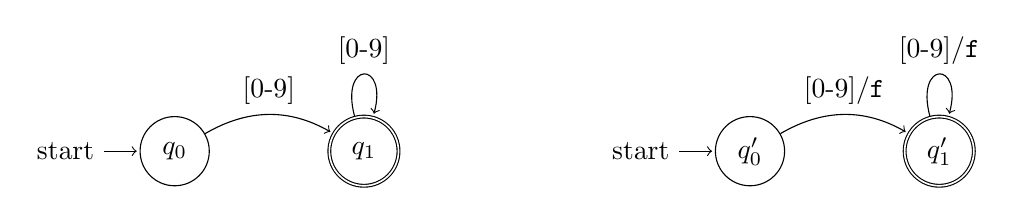
\begin{tikzpicture}[shorten >=1pt, node distance=1.5cm, auto]
  \node[state, initial] (q0)   {$q_0$}; 
  \node[state, accepting] (q1) [right=of q0] {$q_1$}; 

   \path[->] 
   (q0) edge [bend left] node {[0-9]} (q1)
   (q1) edge [loop above] node {[0-9]} (q1);

  \node[state, initial] (q0') [right=4cm of q1] {$q_0'$}; 
  \node[state, accepting] (q1') [right=of q0'] {$q_1'$}; 

   \path[->] 
   (q0') edge [bend left] node {[0-9]/\texttt{f}} (q1')
   (q1') edge [loop above] node {[0-9]/\texttt{f}} (q1');
\end{tikzpicture}
\caption{The SFA for "$[0-9]+$" duplicated}
\label{fig-snfa-pattern}
\end{figure}

\noindent\emph{Step 2.}
The SNFA corresponding to the replacement string "\text{ITP}" is shown in Figure \ref{fig-snfa-replacement}. On the left side is the SFA and on the right side is the corresponding SFT. The function \texttt{g} is the output function that outputs the characters in the replacement string. It can be defined as (the ascii code of $'I'$, $'T'$, $'P'$ are 73, 84, 80 respectively):
\[
\texttt{g} = \lambda~i~x.~\texttt{match }~i~ with~ 1 \rightarrow [(73, 73)] ~|~ 2 \rightarrow [(84, 84)] ~|~ 3 \rightarrow [(80, 80)] ~|~ \_ ~\rightarrow \texttt{None}
\]



\begin{figure}[h] \centering
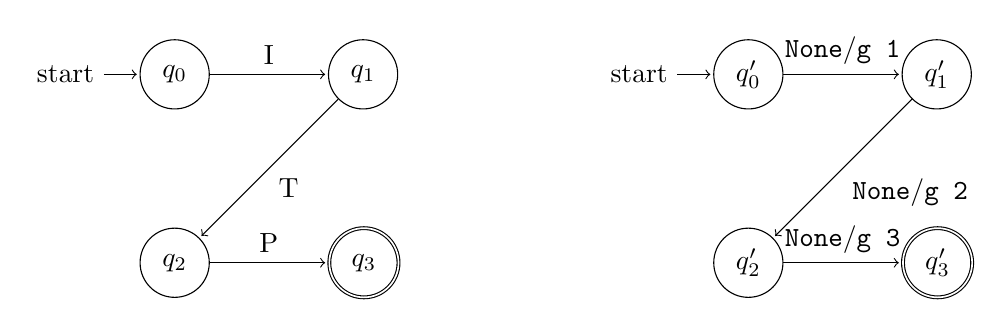
\begin{tikzpicture}[shorten >=1pt, node distance=1.5cm, auto]
  % Original NFA for "ITP"
  \node[state, initial] (q0)   {$q_0$}; 
  \node[state] (q1) [right=of q0] {$q_1$}; 
  \node[state] (q2) [below=of q0] {$q_2$}; 
  \node[state, accepting] (q3) [right=of q2] {$q_3$}; 

  \path[->] 
  (q0) edge node {I} (q1)
  (q1) edge node {T} (q2)
  (q2) edge node {P} (q3);

  % Duplicate NFA for "ITP" on the right
  \node[state, initial] (q0') [right=4cm of q1] {$q_0'$}; 
  \node[state] (q1') [right=of q0'] {$q_1'$}; 
  \node[state] (q2') [below=of q0'] {$q_2'$}; 
  \node[state, accepting] (q3') [right=of q2'] {$q_3'$}; 

  \path[->] 
  (q0') edge node {\texttt{None}/\texttt{g 1}} (q1')
  (q1') edge node {\texttt{None}/\texttt{g 2}} (q2')
  (q2') edge node {\texttt{None}/\texttt{g 3}} (q3');
\end{tikzpicture}
\caption{The SFA for "$"\text{ITP}"$" duplicated}
\label{fig-snfa-replacement}
\end{figure}


\noindent\emph{Step 3.}
The concatenation of the two SFTs is shown in Figure \ref{fig-rearranged-automata}. It contains two minor steps: (1) add a transtion (\texttt{None}/\texttt{f}) from each accepting state of the first SFT to the initial state of the second SFT. (2) add the preceding and succeeding transitions to make it accept the whole input string.

\begin{figure}[h] \centering
  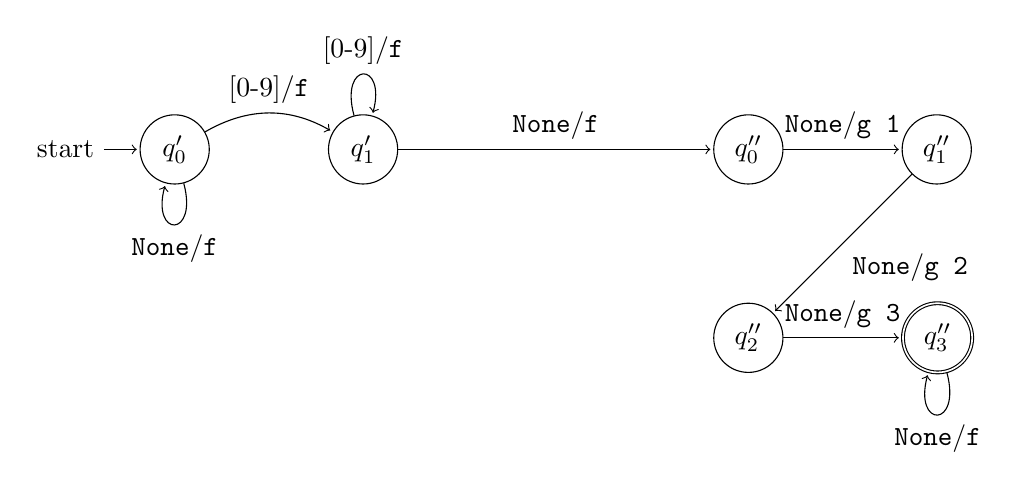
\begin{tikzpicture}[shorten >=1pt, node distance=1.5cm, auto]
    % Second automaton from the first figure
    \node[state, initial] (q0') {$q_0'$}; 
    \node[state] (q1') [right=of q0'] {$q_1'$}; 
  
     \path[->] 
     (q0') edge [bend left] node {[0-9]/\texttt{f}} (q1')
     (q1') edge [loop above] node {[0-9]/\texttt{f}} (q1')
     (q0') edge [loop below] node {\texttt{None}/\texttt{f}} (q0');
  
    % Second automaton from the second figure
    \node[state] (q0'') [right=4cm of q1'] {$q_0''$}; 
    \node[state] (q1'') [right=of q0''] {$q_1''$}; 
    \node[state] (q2'') [below=of q0''] {$q_2''$}; 
    \node[state, accepting] (q3'') [right=of q2''] {$q_3''$}; 
  
    \path[->] 
    (q0'') edge node {\texttt{None}/\texttt{g 1}} (q1'')
    (q1'') edge node {\texttt{None}/\texttt{g 2}} (q2'')
    (q2'') edge node {\texttt{None}/\texttt{g 3}} (q3'')
    (q3'') edge [loop below] node {\texttt{None}/\texttt{f}} (q3'')
    (q1') edge node {\texttt{None}/\texttt{f}} (q0'');
  \end{tikzpicture}
  \caption{The SFT for the replacement operation $\texttt{replace}(s, $"$[0-9]+$"$, $"$\text{ITP}$"$)$}
  \label{fig-rearranged-automata}
  \end{figure}

  With this SFT, we can compute the forward image of the replacement operation.
  Let $s' = \texttt{replace}(s, $"$[0-9]+$"$, $"$\text{ITP}$"$)$ be a string constraint and we want to compute the domain of $s'$ regarding this replacement operation.
  Assume the SFT generated from this replacement operation is $\mathcal{T}$ and the string $s$'s domain ranges over an SFA $\mathcal{A}$. The foward image of this replacement operation is $\mathcal{T}~\mathcal{A}$. Therefore, the domain of $s'$ is $\mathcal{T}~\mathcal{A}$.





\subsection{Experiments}

We have implemented a prototype of the string solver to support the replacement operation based on CertiStr[1], which is called CertiStr-R in this paper.

CertiStr-R supports two kinds of replacement operations: (1) \texttt{str.replace s p r}, where the pattern \texttt{p} is a string and (2) \texttt{str.replace\_re s p r}, where the pattern \texttt{p} is a regular expression. 


The limitation of CertiStr-R is that it does not support \texttt{replace\_all} and \texttt{replace\_re\_all}. CertiStr-R is possible to extend in the future. Another limitation is that the semantics of \texttt{replace} and \texttt{replace\_re} are different from the definition in SMTLIB.

\section{Related Work}

\section{Conclusion}


\bibliography{literature}
\end{document}